% Provenance (never printed): cycle 4 SVT, "La planete Terre, l'environnement":
% glaciers and their landforms, the cryosphere, the glaciations told; see
% sources/book1/PROVENANCE.md. Book 1, grade 8, chapter 5.
% Vocabulary guard: owns glacier; ice sheet + ice shelf + iceberg (one
% definition); sea ice; permafrost; U-shaped valley + moraine (one
% definition); ice age. "Glacial period", "interglacial" and "glacial cycle"
% belong to Book 2 g12 past-climates: here "the ice ages and the warmer times
% between them", in prose. Albedo belongs to Book 2 g10: here "reflects".
% Buoyancy and water expanding as it freezes are physics: recalled in prose.
\chapter{الجليد على الأرض}\label{ch:g8:ice-on-earth}

التُقطت الصورتان أدناه من المكان نفسه، على \omterm{def:g1:landscapes-around-us:water}{بحيرة} ساحلية في ألاسكا، بفارق
26 سنة. ففي عام 1990، كان لسان عريض من الجليد ينزل في \omterm{def:g1:landscapes-around-us:landform}{الوادي} حتى يبلغ الماء.
وفي عام 2016، كان الجليد قد تراجع صعودًا في \omterm{def:g1:landscapes-around-us:landform}{الوادي} وصار أضيق؛ وملأت الأشجار
\omterm{def:g3:stones-pebbles-sand:rock}{والصخور} العارية المكان الذي تركه. وبين عامي 1984 و2021، تبيّن صور الأقمار
الصناعية أن مقدمة هذا \omterm{def:g8:ice-on-earth:glacier}{النهر الجليدي}، \omterm{def:g1:landscapes-around-us:water}{نهر} بيدرسن الجليدي، تراجعت نحو
\qty{3.2}{km}.
% ledger: commons:pedersen, uw:pedersen

\begin{omfigure}
\begin{minipage}[t]{0.49\linewidth}\centering
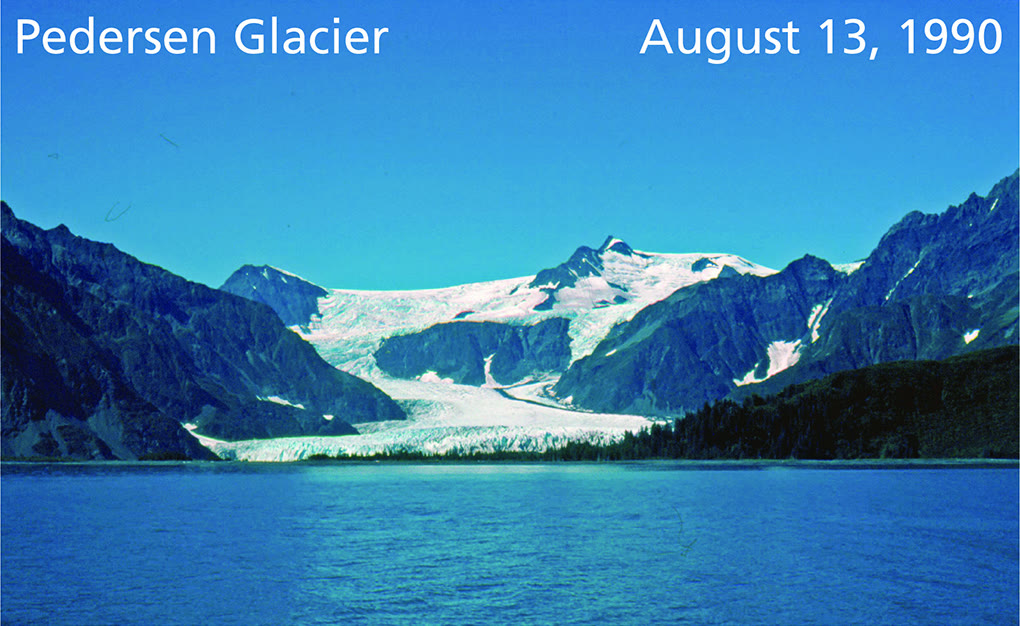
\includegraphics[width=\linewidth]{images/book1/g8-pedersen-1990.jpg}
\end{minipage}\hfill
\begin{minipage}[t]{0.49\linewidth}\centering
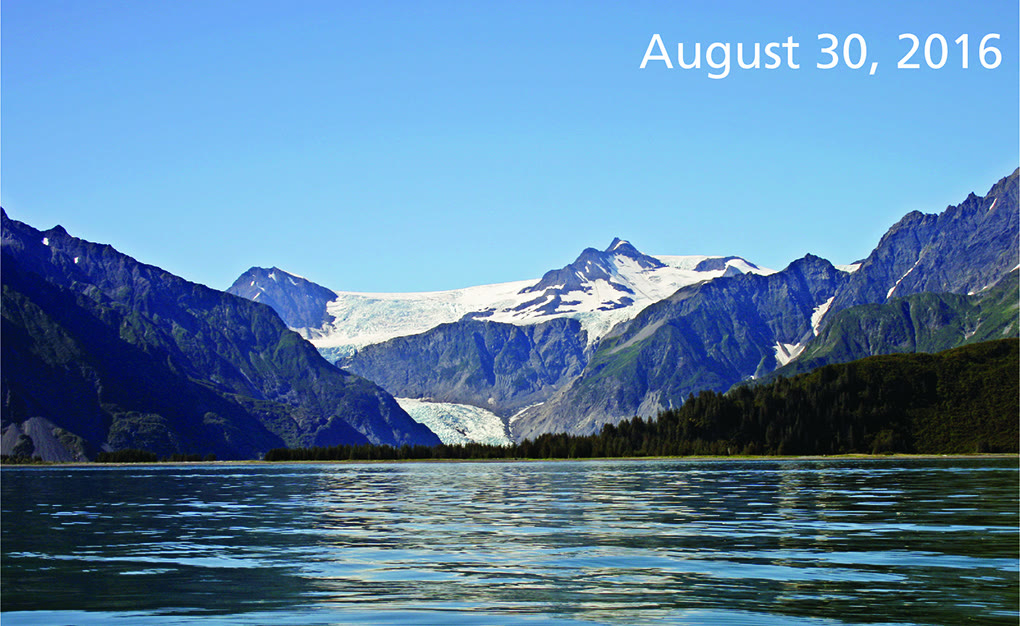
\includegraphics[width=\linewidth]{images/book1/g8-pedersen-2016.jpg}
\end{minipage}

\smallskip
{\small \omterm{def:g1:landscapes-around-us:water}{نهر} بيدرسن الجليدي، متنزه كيناي فيوردز الوطني، ألاسكا، كما يُرى من
المكان نفسه في 13~أغسطس 1990 (يمينًا، تصوير م.~تيترو) وفي 30~أغسطس 2016
(يسارًا، تصوير د.~كورتز). دائرة المتنزهات الوطنية الأمريكية، ملك عام (عبر
ويكيميديا كومنز).}
% ledger: commons:pedersen
\label{fig:g8:ice-on-earth:pedersen}
\end{omfigure}

يغطي الجليد اليوم نحو عُشر اليابسة على الأرض. فهو يقع في \omterm{def:g1:landscapes-around-us:landform}{الأودية} الجبلية، وفي
غطاءين هائلين فوق القارة القطبية الجنوبية وغرينلاند، وعلى البحار القطبية،
ومخبوءًا داخل الأرض المتجمدة في أقصى الشمال. ويتناول هذا الفصل كلًّا منها
بدوره، وكيف يشكّل الجليد سطح الأرض، والأزمنة التي غطى فيها الجليد من الأرض
أكثر بكثير مما يغطيه الآن.
% ledger: nsidc:ice-cover

\begin{recall}
\omterm{def:g4:clouds-rain-snow:precipitation}{الثلج} نوع من \omterm{def:g4:clouds-rain-snow:precipitation}{الهطول}: بلورات جليد تنمو في \omterm{def:g4:clouds-rain-snow:cloud}{سحابة} وتسقط دون أن تذوب
(\cref{ch:g4:clouds-rain-snow}). والماء الجاري يعرّي الأرض، ويحمل القطع بعيدًا
ويرسّبها في مكان أدنى؛ \omterm{def:g1:landscapes-around-us:water}{والنهر} يحفر \omterm{def:g1:landscapes-around-us:landform}{واديًا} (\cref{ch:g5:water-shapes-the-land}).
وحين يتجمد ماء \omterm{def:g2:water-on-earth:ocean}{البحر}، يبقى الملح في الماء \omterm{def:g2:water-on-earth:ocean}{المحيط} بالجليد
(\cref{ch:g8:the-oceans}). وفي الفيزياء تتعلم أن الماء يتمدد حين يتجمد، فيكون
الجليد أقل كثافة من الماء السائل، وأن الجسم الأخف من الماء الذي يزيحه
يطفو.
\end{recall}

\section{الأنهار الجليدية}

عاليًا في \omterm{def:g1:landscapes-around-us:landform}{الجبال}، يسقط في الشتاء من \omterm{def:g4:clouds-rain-snow:precipitation}{الثلج} أكثر مما يذوب في الصيف. وسنة بعد
سنة، يدفن \omterm{def:g4:clouds-rain-snow:precipitation}{الثلج} الجديد \omterm{def:g4:clouds-rain-snow:precipitation}{الثلج} القديم ويضغطه. فتتراص البلورات، ويُعصر الهواء
الذي بينها، وبعد نحو سنة يكون \omterm{def:g4:clouds-rain-snow:precipitation}{الثلج} قد صار \emph{ثلجًا حبيبيًا}، وهو مادة
حبيبية بين \omterm{def:g4:clouds-rain-snow:precipitation}{الثلج} والجليد. ومع دفنه أعمق فأعمق، يتحول \omterm{def:g4:clouds-rain-snow:precipitation}{الثلج} الحبيبي إلى جليد
صلب متماسك؛ ويستغرق ذلك في معظم \omterm{def:g8:ice-on-earth:glacier}{الأنهار الجليدية} أكثر من مئة سنة.
% ledger: nsidc:firn

\begin{definition}[النهر الجليدي]\label{def:g8:ice-on-earth:glacier}
\emph{النهر الجليدي}\index{نهر جليدي} كتلة من الجليد، تكونت من \omterm{def:g4:clouds-rain-snow:precipitation}{ثلج} تراكم على
مدى سنين كثيرة، تتحرك ببطء نحو أسفل المنحدر فوق اليابسة بفعل وزنها.
\end{definition}
% ledger: nsidc:glacier-def

\omterm{def:g8:ice-on-earth:glacier}{للنهر الجليدي} جزءان. ففي جزئه الأعلى، أي \emph{منطقة التراكم}، يسقط كل سنة
من \omterm{def:g4:clouds-rain-snow:precipitation}{الثلج} أكثر مما يذوب: فيكسب \omterm{def:g8:ice-on-earth:glacier}{النهر الجليدي} جليدًا. وفي جزئه الأدنى، أي
\emph{منطقة الذوبان}، يذوب كل سنة من الجليد أكثر مما يسقط من \omterm{def:g4:clouds-rain-snow:precipitation}{الثلج}: فيخسر
\omterm{def:g8:ice-on-earth:glacier}{النهر الجليدي} جليدًا. ويظل الجليد المكتسب في الأعلى يجري نحو الأسفل ليعوّض
الجليد المفقود في الأسفل. فإذا تعادل الاثنان، بقي طرف \omterm{def:g8:ice-on-earth:glacier}{النهر الجليدي} الأمامي،
أي \emph{مقدمته}، في المكان نفسه.
% ledger: nsidc:glacier-zones

\begin{omfigure}
\begin{tikzpicture}[font=\footnotesize, >={Stealth[length=2mm]}, xscale=1.08]
  % bedrock
  \fill[black!13] (0,4.6) -- (2,3.9) -- (4,3.0) -- (6,2.0) -- (8,1.1)
    -- (10,0.45) -- (11,0.3) -- (13,0.15) -- (13,-0.5) -- (0,-0.5) -- cycle;
  % the ice body, two zones
  \begin{scope}
    \clip (0,5.5) -- (2,4.9) -- (4,4.0) -- (6,2.9) -- (8,1.8) -- (9.4,0.95)
      -- (10,0.45) -- (8,1.1) -- (6,2.0) -- (4,3.0) -- (2,3.9) -- (0,4.6) -- cycle;
    \fill[omIce] (0,-1) rectangle (5,6);
    \fill[omSea!85] (5,-1) rectangle (11,6);
  \end{scope}
  \draw[black!60] (0,5.5) -- (2,4.9) -- (4,4.0) -- (6,2.9) -- (8,1.8)
    -- (9.4,0.95) -- (10,0.45);
  \draw[black!70, line width=0.6pt] (0,4.6) -- (2,3.9) -- (4,3.0) -- (6,2.0)
    -- (8,1.1) -- (10,0.45) -- (11,0.3) -- (13,0.15);
  % snowline
  \draw[dashed, black!70] (5,2.5) -- (5,4.15);
  \node[anchor=south] at (5,4.15) {تساقط الثلج = الذوبان};
  % snowflakes and melting
  \foreach \x/\y in {0.5/6.1, 1.3/5.8, 2.1/5.5, 2.9/5.1, 3.7/4.8, 0.9/6.6, 1.7/6.3, 2.5/6.0, 3.3/5.6, 4.1/5.2}
    \node[omCold] at (\x,\y) {$\ast$};
  \foreach \x/\y in {6.4/2.8, 7.2/2.35, 8.0/1.9}
    \draw[omWarm, decorate, decoration={snake, amplitude=0.6mm, segment length=2mm}] (\x,\y) -- ++(0,0.6);
  % flow arrows inside the ice
  \draw[->, omDef, line width=0.9pt] (1.0,4.72) -- (2.2,4.30);
  \draw[->, omDef, line width=0.9pt] (3.0,3.95) -- (4.2,3.41);
  \draw[->, omDef, line width=0.9pt] (5.2,2.88) -- (6.4,2.28);
  \draw[->, omDef, line width=0.9pt] (7.2,1.84) -- (8.3,1.35);
  % moraine and meltwater
  \fill[omLithCongl] (10.15,0.42) .. controls (10.5,0.95) and (10.9,0.95) .. (11.2,0.29) -- cycle;
  \draw[omSea!60!black, line width=1.6pt] (10.05,0.38) .. controls (10.6,0.22) and (11.4,0.12) .. (12.9,0.08);
  % labels
  \node[align=center] at (1.9,7.15) {\textbf{منطقة التراكم}\\ يتراكم الثلج ويكسب النهر الجليدي جليدًا};
  \node[align=center] at (10.0,3.3) {\textbf{منطقة الذوبان}\\ يذوب الجليد ويخسر النهر الجليدي جليدًا};
  \node[align=left, anchor=west, omDef] at (4.4,1.3) {يجري الجليد\\ نحو الأسفل};
  \draw[black!60] (10.0,0.5) -- (9.6,-0.1) node[below] {المقدمة};
  \draw[black!60] (10.7,0.85) -- (11.3,1.4) node[above] {ركام جليدي};
  \node[anchor=north east] at (12.9,0.0) {مجرى ماء الذوبان};
  \node at (2.2,2.6) {الصخر الأساسي};
\end{tikzpicture}

{\small \omterm{def:g8:ice-on-earth:glacier}{نهر جليدي} في \omterm{def:g1:landscapes-around-us:landform}{وادٍ}، في مقطع طولي (رسم تخطيطي، ليس بمقياس رسم). فوق
الخط المتقطع، يتراكم \omterm{def:g4:clouds-rain-snow:precipitation}{الثلج} أسرع مما يذوب؛ وتحته، يذوب الجليد أسرع مما يسقط
\omterm{def:g4:clouds-rain-snow:precipitation}{الثلج}. ويجري الجليد نزولًا من جزء إلى الآخر.}
\label{fig:g8:ice-on-earth:long-section}
\end{omfigure}

كيف يمكن لجليد صلب أن يجري؟ تحت وزن الجليد الذي فوقه، يتشوه الجليد العميق في
\omterm{def:g8:ice-on-earth:glacier}{النهر الجليدي} ببطء، كما تنتشر طبقة سميكة من العسل البارد. وينزلق \omterm{def:g8:ice-on-earth:glacier}{النهر الجليدي}
أيضًا فوق \omterm{def:g3:stones-pebbles-sand:rock}{الصخر} الذي تحته، على غشاء رقيق من الماء أو على \omterm{def:g3:stones-pebbles-sand:sand}{وحل} مبلل. وقاع \omterm{def:g8:ice-on-earth:glacier}{النهر
الجليدي}، باحتكاكه \omterm{def:g3:stones-pebbles-sand:rock}{بالصخر}، يتحرك أبطأ من سطحه. ومعظم \omterm{def:g8:ice-on-earth:glacier}{الأنهار الجليدية} تتحرك
ببطء وانتظام؛ وقليل منها \emph{يندفع} فجأة. ففي عام 1986، اندفع \omterm{def:g1:landscapes-around-us:water}{نهر} هبارد
الجليدي في ألاسكا إلى الأمام نحو \qty{10}{m} في اليوم، وأسرع اندفاع مسجّل،
\omterm{def:g1:landscapes-around-us:water}{لنهر} كوتياه الجليدي في باكستان عام 1953، بلغ متوسطه نحو \qty{112}{m} في اليوم
طوال ثلاثة أشهر.
% ledger: nsidc:glacier-flow, nsidc:surges

حين يخسر \omterm{def:g8:ice-on-earth:glacier}{النهر الجليدي} في الأسفل من الجليد أكثر مما يكسبه في الأعلى، تتراجع
مقدمته صعودًا في \omterm{def:g1:landscapes-around-us:landform}{الوادي}: \omterm{def:g8:ice-on-earth:glacier}{فالنهر الجليدي} \emph{يتراجع}. \omterm{def:g8:ice-on-earth:glacier}{والنهر الجليدي} المتراجع
لا يزال يجري نحو الأسفل، كحزام ناقل؛ لكنه يذوب أسرع مما يجري. وكان \omterm{def:g1:landscapes-around-us:water}{نهر} ميوير
الجليدي، في ألاسكا، يملأ واديه كله حتى \omterm{def:g2:water-on-earth:ocean}{البحر} عام 1941. وبحلول عام 2004، كانت
مقدمته قد تراجعت \qty{12}{km}، وانخفض سطح الجليد بأكثر من
\qty{800}{m}.
% ledger: nsidc:glacier-flow, nsidc:muir

\section{كيف يشكّل الجليد واديًا}

\omterm{def:g8:ice-on-earth:glacier}{النهر الجليدي} أداة \omterm{def:g5:water-shapes-the-land:erosion}{تعرية} قوية. فجليده يتجمد على كتل \omterm{def:g3:stones-pebbles-sand:rock}{الصخر} المفككة ويقتلعها؛
والحجارة المتجمدة في قاعدته تكشط \omterm{def:g3:stones-pebbles-sand:rock}{الصخر} الذي تحته كورق الصنفرة. ويحمل \omterm{def:g8:ice-on-earth:glacier}{النهر
الجليدي} كل هذا \omterm{def:g3:stones-pebbles-sand:rock}{الصخر}، من الغبار الناعم إلى الجلاميد الضخمة، نزولًا في \omterm{def:g1:landscapes-around-us:landform}{الوادي}
كحزام ناقل، ويلقيه حيث يذوب الجليد.
% ledger: nps:u-valley

\begin{omfigure}
\begin{tikzpicture}[font=\footnotesize, >={Stealth[length=2mm]}]
  % V-shaped valley
  \fill[black!13] (0,3) -- (2.1,0.35) -- (2.5,0.35) -- (4.6,3) -- (4.6,-0.4) -- (0,-0.4) -- cycle;
  \draw[black!70, line width=0.6pt] (0,3) -- (2.1,0.35) -- (2.5,0.35) -- (4.6,3);
  \fill[omSea] (2.1,0.35) -- (2.5,0.35) -- (2.42,0.2) -- (2.18,0.2) -- cycle;
  \node[align=center] at (2.3,-0.85) {نهر يحفر واديًا ضيقًا\\ \foreignlanguage{arabic}{على شكل حرف V}};
  % arrow
  \draw[->, line width=1pt] (5.0,1.5) -- (6.2,1.5) node[midway, above, align=center] {يملؤه\\ نهر جليدي};
  % U-shaped valley
  \begin{scope}[xshift=6.6cm]
    \fill[black!13] (0,3) .. controls (0.6,1.0) and (0.9,0.25) .. (1.6,0.2)
      -- (3.0,0.2) .. controls (3.7,0.25) and (4.0,1.0) .. (4.6,3) -- (4.6,-0.4) -- (0,-0.4) -- cycle;
    \draw[black!70, line width=0.6pt] (0,3) .. controls (0.6,1.0) and (0.9,0.25) .. (1.6,0.2)
      -- (3.0,0.2) .. controls (3.7,0.25) and (4.0,1.0) .. (4.6,3);
    \draw[dashed, black!40] (0,3) -- (2.1,0.35) -- (2.5,0.35) -- (4.6,3);
    \draw[omCold, line width=0.9pt] (0.37,2.2) -- (4.23,2.2);
    \node[omCold, anchor=south, font=\scriptsize] at (2.3,2.2) {سطح الجليد قديمًا};
    \fill[omLithCongl] (0.75,0.95) .. controls (0.95,1.2) and (1.1,1.1) .. (1.2,0.6) -- cycle;
    \fill[omLithCongl] (3.85,0.95) .. controls (3.65,1.2) and (3.5,1.1) .. (3.4,0.6) -- cycle;
    \node[align=center] at (2.3,-0.85) {بعد زوال الجليد وادٍ عريض\\ \foreignlanguage{arabic}{على شكل حرف U، جوانبه شديدة الانحدار}};
    \draw[black!60] (3.65,0.95) -- (4.85,0.6) node[right, align=left] {ركام جليدي\\ جانبي};
    \node[font=\scriptsize, black!55, align=center] at (2.3,1.6) {\foreignlanguage{arabic}{الوادي \babelsublr{V} القديم متقطع}};
  \end{scope}
\end{tikzpicture}

{\small \omterm{def:g1:landscapes-around-us:landform}{الوادي} الجبلي نفسه في مقطع عرضي، قبل \omterm{def:g8:ice-on-earth:glacier}{النهر الجليدي} وبعده (رسم
تخطيطي). يكشط الجليد \omterm{def:g1:landscapes-around-us:landform}{الوادي} النهري الضيق فيجعله حوضًا عريضًا له قاع واسع
وجوانب شديدة الانحدار، ويترك على حوافه حواجز مرتفعة من الحطام
الصخري.}
\label{fig:g8:ice-on-earth:v-and-u}
\end{omfigure}

\begin{definition}[الوادي على شكل حرف U والركام الجليدي]\label{def:g8:ice-on-earth:glacial-landforms}
\emph{الوادي على شكل حرف U}\index{وادٍ على شكل حرف U} \omterm{def:g1:landscapes-around-us:landform}{وادٍ} له قاع عريض مستوٍ وجوانب
شديدة الانحدار، نحته \omterm{def:g8:ice-on-earth:glacier}{نهر جليدي} وسّع \omterm{def:g1:landscapes-around-us:landform}{واديًا} نهريًا ضيقًا على شكل حرف V
وعمّقه. و\emph{الركام الجليدي}\index{ركام جليدي} حاجز مرتفع من الحطام الصخري، من الغبار إلى
الجلاميد، يتركه \omterm{def:g8:ice-on-earth:glacier}{نهر جليدي}: \emph{ركام جليدي جانبي} على طول جانبه،
و\emph{ركام جليدي طرفي} عند نهايته.
\end{definition}
% ledger: usgs:erratic, nps:u-valley, nps:moraines

الركامات الجليدية دلائل مفيدة. \omterm{def:g8:ice-on-earth:glacial-landforms}{فالركام الجليدي} الطرفي البعيد في أسفل \omterm{def:g1:landscapes-around-us:landform}{الوادي}،
ولا جليد في أي مكان قريب منه، يبين إلى أي مدى بلغ \omterm{def:g8:ice-on-earth:glacier}{النهر الجليدي} يومًا؛
\omterm{def:g8:ice-on-earth:glacial-landforms}{والركام الجليدي} الجانبي العالي على جانب \omterm{def:g1:landscapes-around-us:landform}{الوادي} يبين كم كان سُمك الجليد يومًا.
والجلمود الكبير القابع وحده في حقل، المكوَّن من \omterm{def:g3:stones-pebbles-sand:rock}{صخر} لا يوجد في أي مكان قريب،
دليل آخر: إنه \emph{صخرة ضالة}، أي صخرة حملها \omterm{def:g8:ice-on-earth:glacier}{نهر جليدي} بعيدًا عن موطنها
وتركها حين ذاب الجليد. وتتراوح \omterm{def:g3:stones-pebbles-sand:rock}{الصخور} الضالة بين \omterm{def:g3:stones-pebbles-sand:pebble}{الحصى} وكتل أكبر من
بيت.
% ledger: nps:moraines, usgs:erratic

\begin{inthefield}[قراءة وادٍ شكّله الجليد]
في نزهة في \omterm{def:g1:landscapes-around-us:landform}{الجبال}، أو في صورة \omterm{def:g1:landscapes-around-us:landform}{لوادٍ} جبلي، انظر إلى شكل \omterm{def:g1:landscapes-around-us:landform}{الوادي} في مقطع عرضي:
أهو حرف V ضيق، أم حرف U عريض جدرانه شديدة الانحدار؟ وابحث في قاع \omterm{def:g1:landscapes-around-us:landform}{الوادي} عن
حواجز طويلة من الحجارة والتراب المختلطة تمتد على طول جوانبه أو تعترضه: فقد
تكون ركامات جليدية. وابحث عن جلاميد كبيرة لا تشبه \omterm{def:g3:stones-pebbles-sand:rock}{الصخر} \omterm{def:g2:water-on-earth:ocean}{المحيط} بها، وعن أسطح
صخرية ملساء تخدشها خطوط طويلة متوازية. والزم الممرات، وابتعد عن حواف
المنحدرات الشديدة وعن الجليد نفسه، وارسم ما تراه في
دفترك.
\end{inthefield}

\section{الأغطية الجليدية والرفوف الجليدية والجبال الجليدية}

أكبر كتل الجليد على الأرض ليست في \omterm{def:g1:landscapes-around-us:landform}{الأودية} الجبلية: إنها تغطي أراضي بأكملها.
\omterm{def:g8:ice-on-earth:ice-sheet}{فالغطاء الجليدي} \omterm{def:g3:continents-and-oceans:continent}{للقارة} القطبية الجنوبية يمتد على قرابة
\num{14}~مليون~\unit{km^2}، ويبلغ سُمكه نحو \qty{4.9}{km} في أسمك مواضعه.
ويغطي \omterm{def:g8:ice-on-earth:ice-sheet}{الغطاء الجليدي} لغرينلاند نحو \num{1.7}~مليون~\unit{km^2}، أي أربعة أخماس
الجزيرة، ويزيد سُمكه على \qty{3}{km}. ويحتويان معًا أكثر من 99~\% من الجليد
على اليابسة، وأكثر من ثلثي \omterm{def:g2:water-on-earth:salt-fresh}{الماء العذب} كله على
الأرض.
% ledger: nsidc:ice-sheets

\begin{definition}[الغطاء الجليدي والرف الجليدي والجبل الجليدي]\label{def:g8:ice-on-earth:ice-sheet}
\emph{الغطاء الجليدي}\index{غطاء جليدي} كتلة من الجليد تغطي أكثر من
\qty{50000}{km^2} من اليابسة، كقبة هائلة تنتشر نحو الخارج في كل الاتجاهات.
وحيث يبلغ الجليد الجاري من اليابسة \omterm{def:g2:water-on-earth:ocean}{البحر} ويواصل الطفو عليه، وهو لا يزال
متصلًا بالجليد الذي خلفه، يكوّن \emph{رفًّا جليديًا}\index{رف جليدي}.
و\emph{الجبل الجليدي}\index{جبل جليدي} كتلة كبيرة من الجليد، يزيد عرضها على \qty{5}{m}،
انفصلت عن \omterm{def:g8:ice-on-earth:glacier}{نهر جليدي} أو عن رف جليدي وتطفو في
\omterm{def:g2:water-on-earth:ocean}{البحر}.
\end{definition}
% ledger: nsidc:ice-sheets, nsidc:ice-shelves, nsidc:iceberg

\begin{omfigure}
\begin{minipage}[c]{0.5\linewidth}\centering
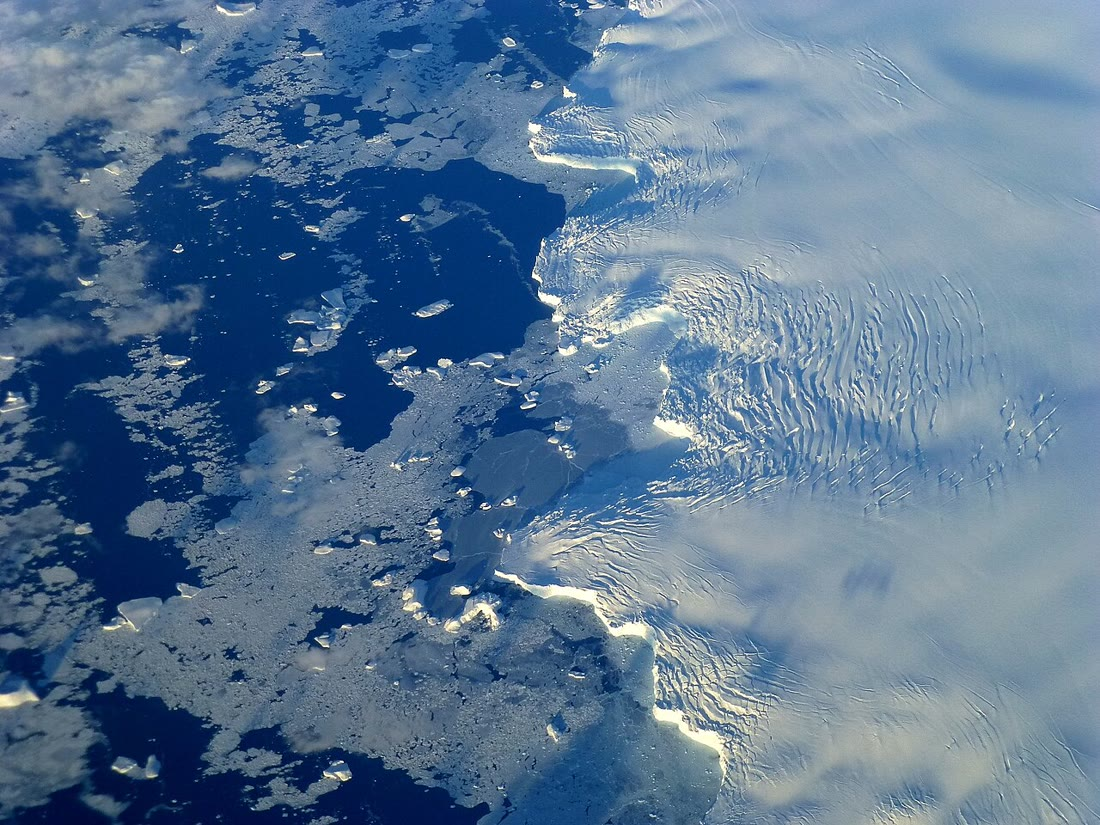
\includegraphics[width=\linewidth]{images/book1/g8-ice-shelf-edge.jpg}
\end{minipage}\hfill
\begin{minipage}[c]{0.46\linewidth}\raggedright
{\small حافة \omterm{def:g8:ice-on-earth:ice-sheet}{رف جليدي} قرب جزيرة أديلايد، قبالة شبه الجزيرة القطبية الجنوبية،
كما تُرى من طائرة في 28~أكتوبر 2012. الجليد الأبيض السميك المجعّد على اليمين
هو \omterm{def:g8:ice-on-earth:ice-sheet}{الرف الجليدي}؛ وعلى اليسار تطفو قطع مكسرة من \omterm{def:g8:ice-on-earth:sea-ice}{جليد بحري} أرق على الماء
الداكن. ناسا، عملية آيس بريدج (ملك عام، عبر ويكيميديا
كومنز).}
\end{minipage}
% ledger: commons:ice-shelf
\label{fig:g8:ice-on-earth:ice-shelf}
\end{omfigure}

الماء المحبوس في \omterm{def:g8:ice-on-earth:ice-sheet}{الأغطية الجليدية} جاء من \omterm{def:g2:water-on-earth:ocean}{المحيط}: فقد تبخر، وسقط ثلجًا وتراكم
على اليابسة. ولو ذاب كل جليد غرينلاند، لارتفع \omterm{def:g2:water-on-earth:ocean}{البحر} نحو \qty{7.4}{m}؛ ولو ذاب
كل جليد القارة القطبية الجنوبية، لارتفع نحو \qty{58}{m}. أما \omterm{def:g8:ice-on-earth:glacier}{الأنهار الجليدية}
الجبلية في العالم كله، وعددها أكثر من \num{200000}، فلن تضيف إلا أقل من نصف
متر.
% ledger: nsidc:ice-sheets, nsidc:ice-cover

\begin{omfigure}
\begin{tikzpicture}
\begin{axis}[omrecord, xbar, width=10.5cm, height=3.6cm, xmin=0, xmax=68,
  bar width=9pt, ytick=data, symbolic y coords={glaciers,Greenland,Antarctica},
  yticklabels={كل الأنهار الجليدية الجبلية, الغطاء الجليدي لغرينلاند, الغطاء الجليدي للقارة القطبية الجنوبية},
  xlabel={\foreignlanguage{arabic}{ارتفاع البحر لو ذاب كله \babelsublr{(m)}}}, enlarge y limits=0.3,
  nodes near coords, nodes near coords style={font=\footnotesize, anchor=west, fill=white, inner sep=1.5pt},
  ymajorgrids=false]
  \addplot[fill=omIce!80!black, draw=black!60] coordinates {(0.5,glaciers) (7.4,Greenland) (58,Antarctica)};
\end{axis}
\end{tikzpicture}

{\small مقدار ارتفاع البحر لو ذاب كل نوع من جليد اليابسة ذوبانًا تامًا (القيم
من المركز الوطني لبيانات \omterm{def:g4:clouds-rain-snow:precipitation}{الثلج} والجليد؛ وقيمة \omterm{def:g8:ice-on-earth:glacier}{الأنهار الجليدية} حد أعلى،
«أقل بقليل من نصف متر»).}
% ledger: nsidc:ice-sheets, nsidc:ice-cover
\label{fig:g8:ice-on-earth:sea-level-bars}
\end{omfigure}

أما الجليد الطافي فأمره مختلف. \omterm{def:g8:ice-on-earth:ice-sheet}{فالرف الجليدي} أو \omterm{def:g8:ice-on-earth:ice-sheet}{الجبل الجليدي} يطفو على \omterm{def:g2:water-on-earth:ocean}{البحر}
أصلًا: فقد أزاح من قبلُ ماءً يعادل وزنه. وحين يتكسر أو يذوب، لا يرتفع \omterm{def:g2:water-on-earth:ocean}{البحر}.
لكن \omterm{def:g8:ice-on-earth:ice-sheet}{الرف الجليدي} يحجز \omterm{def:g8:ice-on-earth:glacier}{الأنهار الجليدية} التي خلفه، كالسدادة في القارورة؛ وحين
تفكك \omterm{def:g8:ice-on-earth:ice-sheet}{الرف الجليدي} لارسن~B في القارة القطبية الجنوبية عام 2002، تسارعت \omterm{def:g8:ice-on-earth:glacier}{الأنهار
الجليدية} التي خلفه، وبلغ بعضها ثمانية أضعاف سرعته السابقة، وصبّت في \omterm{def:g2:water-on-earth:ocean}{البحر}
مزيدًا من جليد اليابسة.
% ledger: nsidc:ice-shelves

\begin{inthelab}[جليد طافٍ وجليد على اليابسة]
داخل البيت، ضع حجرًا صغيرًا في كل من كأسين شفافتين بحيث يبرز فوق الماء حين
تملؤهما. في الكأس الأولى، اجعل بضعة مكعبات من الجليد تطفو على الماء. وفي
الثانية، ضع العدد نفسه من مكعبات الجليد على الحجر، خارج الماء. املأ الكأسين
بالماء إلى المستوى نفسه وعلّمه بقلم لبّاد. انتظر حتى يذوب الجليد كله، ثم قارن
مستويي الماء بالعلامتين. أي الكأسين تتصرف مثل \omterm{def:g2:water-on-earth:ocean}{البحر} حين يذوب \omterm{def:g8:ice-on-earth:ice-sheet}{جبل جليدي}،
وأيهما مثل \omterm{def:g2:water-on-earth:ocean}{البحر} حين يذوب \omterm{def:g8:ice-on-earth:ice-sheet}{غطاء جليدي}؟
\end{inthelab}

\section{الجليد البحري}

\omterm{def:g8:ice-on-earth:sea-ice}{الجليد البحري} شيء آخر أيضًا: إنه \omterm{def:g2:water-on-earth:ocean}{البحر} نفسه وقد تجمد. ففي كل شتاء يتجمد سطح
المحيطات القطبية على مساحة شاسعة؛ وفي كل صيف يذوب كثير من هذا الجليد من جديد.
وفي المنطقة القطبية الشمالية، يكون الجليد في أصغر امتداد له في نهاية الصيف، في
سبتمبر، وفي أكبر امتداد له في نهاية الشتاء، في مارس. وقد قاست الأقمار الصناعية
\emph{امتداده}، أي مساحة \omterm{def:g2:water-on-earth:ocean}{البحر} التي يغطي الجليد 15~\% على الأقل من سطحها، كل
يوم منذ أواخر سبعينيات القرن العشرين.
% ledger: nsidc:sea-ice-def

\begin{definition}[الجليد البحري]\label{def:g8:ice-on-earth:sea-ice}
\emph{الجليد البحري}\index{جليد بحري} ماء \omterm{def:g2:water-on-earth:ocean}{بحر} متجمد: يتكون وينمو ويذوب في
\omterm{def:g2:water-on-earth:ocean}{المحيط} نفسه. وهو يختلف عن \omterm{def:g1:landscapes-around-us:landform}{الجبال} الجليدية \omterm{def:g8:ice-on-earth:ice-sheet}{والرفوف الجليدية}، التي تطفو على
\omterm{def:g2:water-on-earth:ocean}{البحر} لكنها تكونت من \omterm{def:g4:clouds-rain-snow:precipitation}{ثلج} سقط على اليابسة.
\end{definition}
% ledger: nsidc:sea-ice-def

\omterm{def:g8:ice-on-earth:sea-ice}{للجليد البحري} أهمية تتجاوز \omterm{def:g3:continents-and-oceans:poles}{القطبين} بكثير. فماء \omterm{def:g2:water-on-earth:ocean}{البحر} المكشوف داكن: لا يعكس إلا
نحو 6~\% من ضوء الشمس الذي يبلغه ويمتص الباقي. أما \omterm{def:g8:ice-on-earth:sea-ice}{الجليد البحري} فيعكس من 50
إلى 70~\%، \omterm{def:g8:ice-on-earth:sea-ice}{والجليد البحري} المغطى \omterm{def:g4:clouds-rain-snow:precipitation}{بالثلج} حتى 90~\%. وحين يذوب الجليد، يمتص الماء
الداكن الذي تحته مزيدًا من طاقة الشمس ويسخن، فيذيب مزيدًا من
الجليد.
% ledger: nsidc:sea-ice-reflect

\begin{omfigure}
\begin{tikzpicture}
\begin{axis}[omrecord, width=13cm, height=5.4cm, xmin=1977, xmax=2027,
  ymin=3, ymax=8.2, xtick={1980,1990,...,2020},
  x tick label style={/pgf/number format/1000 sep={}},
  xlabel={\foreignlanguage{arabic}{السنة}}, ylabel={\foreignlanguage{arabic}{الامتداد بملايين \babelsublr{km$^2$}}},
  legend style={at={(0.98,0.97)}, anchor=north east, draw=none, fill=white}]
  \addplot[omCold, mark=*, mark size=1.3pt, line width=0.6pt]
    table[x=year, y=extent_Mkm2] {figdata/out/grade-8-sea_ice-extent.dat};
  \addlegendentry{\foreignlanguage{arabic}{متوسط الامتداد في سبتمبر}}
  \addplot[omWarm, dashed, line width=1pt]
    table[x=year, y=extent_Mkm2] {figdata/out/grade-8-sea_ice-trend.dat};
  \addlegendentry{\foreignlanguage{arabic}{خط الاتجاه}}
  \node[font=\scriptsize, anchor=north] at (axis cs:2012,3.5) {2012};
\end{axis}
\end{tikzpicture}

{\small امتداد \omterm{def:g8:ice-on-earth:sea-ice}{الجليد البحري} في المنطقة القطبية الشمالية في كل سبتمبر،
1979--2025، والخط المستقيم الذي يتبع النقاط على أفضل وجه. البيانات: مؤشر
\omterm{def:g8:ice-on-earth:sea-ice}{الجليد البحري} للمركز الوطني لبيانات \omterm{def:g4:clouds-rain-snow:precipitation}{الثلج} والجليد، الإصدار~4 (ف.~فيتيرر
وآخرون، 2025).}
% ledger: data:b1-nsidc-sea-ice (figdata/grade-8/sea_ice.py)
\label{fig:g8:ice-on-earth:sea-ice}
\end{omfigure}

تصعد النقاط وتهبط من سنة إلى التي تليها: \omterm{def:g1:watching-the-weather:weather}{فطقس} كل صيف له أثره. لكنها على مر
السنين تنخفض بوضوح. ولرؤية التغير عبر الصعود والهبوط، يرسم العلماء \emph{خط
الاتجاه}، وهو الخط المستقيم الذي يمر بأقرب ما يمكن من النقاط
كلها.
% ledger: data:b1-nsidc-sea-ice (figdata/grade-8/sea_ice.py)

\begin{method}[قراءة اتجاه على مخطط بياني]
\begin{enumerate}
  \item اقرأ المحورين: ما الذي يُقاس، وبأي وحدة، وعلى مدى أي سنوات.
  \item انظر إلى النقاط: هل وراء الصعود والهبوط ارتفاع عام، أم انخفاض
        عام، أم لا هذا ولا ذاك؟
  \item اقرأ خط الاتجاه عند السنة الأولى وعند السنة الأخيرة.
  \item خذ الفرق، واقسمه على عدد السنوات (أو العقود) بينهما: فهذا هو
        متوسط التغير في السنة (أو في العقد).
  \item لا تستنتج الكثير من سنة واحدة: فالنقطة الوحيدة البعيدة عن
        الخط \omterm{def:g1:watching-the-weather:weather}{طقس}، والخط هو الاتجاه.
\end{enumerate}
\end{method}

\begin{example}[جليد سبتمبر في المنطقة القطبية الشمالية]
على المخطط، يقع خط الاتجاه عند نحو \num{7.6}~مليون~\unit{km^2} عام 1979
وعند نحو \num{4.1}~مليون~\unit{km^2} عام 2025. فالتغير هو $7.6 - 4.1 =
3.5$ مليون~\babelsublr{km$^2$} في $2025 - 1979 = 46$ سنة، أي 4.6 عقود:
$3.5 \div 4.6 \approx 0.76$. فقد تقلص جليد سبتمبر البحري بنحو
\num{0.76}~مليون~\unit{km^2} في كل عقد: وفي 46 سنة، فقد خط الاتجاه قرابة نصف
قيمته عام 1979. وأدنى نقطة، \num{3.57}~مليون~\unit{km^2} عام 2012، تقع تحت
الخط بكثير: فقد كان ذلك الصيف استثنائيًا.
\end{example}
% ledger: data:b1-nsidc-sea-ice (figdata/grade-8/sea_ice.py), nsidc:sea-ice-reflect

تبين القياسات أن جليد الصيف البحري في المنطقة القطبية الشمالية قد صار أصغر
وأرق معًا منذ ثمانينيات القرن العشرين، مع احترار المنطقة القطبية الشمالية.
ويتناول \Cref{ch:g9:climate-past-and-present} كيف يتغير \omterm{def:g5:weather-and-climate:climate}{مناخ} الأرض،
ولماذا.
% ledger: nsidc:sea-ice-reflect

\section{التربة الصقيعية}

في أقصى الشمال، يتغلغل الصقيع عميقًا في الأرض. فتحت تندرا أمريكا الشمالية
وغرينلاند وشمال آسيا، تبقى التربة \omterm{def:g3:stones-pebbles-sand:rock}{والصخر} متجمدة طوال السنة، وكثيرًا ما تكون
متجمدة منذ آلاف السنين. ولا تذوب كل صيف وتتجمد من جديد كل شتاء إلا طبقة علوية
رقيقة، هي \emph{الطبقة النشطة}؛ تنمو فيها النباتات، والماء الذي لا يستطيع
\omterm{def:g6:water-underground:infiltration}{التسرب} إلى الأرض المتجمدة تحتها يتجمع في برك على السطح.
% ledger: nsidc:permafrost

\begin{definition}[التربة الصقيعية]\label{def:g8:ice-on-earth:permafrost}
\emph{التربة الصقيعية}\index{تربة صقيعية} أرض، تربةً كانت أو \omterm{def:g3:stones-pebbles-sand:rock}{صخرًا}، تبقى عند
\qty{0}{\degreeCelsius} أو دونها مدة سنتين متتاليتين على الأقل.
\end{definition}
% ledger: nsidc:permafrost

تقع \omterm{def:g8:ice-on-earth:permafrost}{التربة الصقيعية} تحت نحو \num{23}~مليون~\unit{km^2}، أي ربع يابسة \omterm{def:g3:continents-and-oceans:equator}{نصف الكرة
الشمالي}، وتحت نحو 85~\% من ألاسكا. والأرض المتجمدة المليئة بالجليد صلبة
\omterm{def:g3:stones-pebbles-sand:rock}{كالصخر}؛ وحين يذوب جليدها، تتحول الأرض إلى \omterm{def:g3:stones-pebbles-sand:sand}{وحل} وتهبط. فتتشقق الطرق، وتميل
المباني، وقد تنكسر خطوط الأنابيب: فحيث يعبر خط أنابيب عبر ألاسكا \omterm{def:g8:ice-on-earth:permafrost}{التربة
الصقيعية}، يمتد فوق الأرض مسافة \qty{676}{km}. كما أن ذوبان \omterm{def:g8:ice-on-earth:permafrost}{التربة الصقيعية}
يسمح لبقايا النباتات المتجمدة فيها منذ آلاف السنين بأن تتحلل، فتطلق ثاني
أكسيد الكربون والميثان في الهواء.
% ledger: nsidc:permafrost, nsidc:permafrost-thaw

\begin{omfigure}
\begin{minipage}[c]{0.5\linewidth}\centering
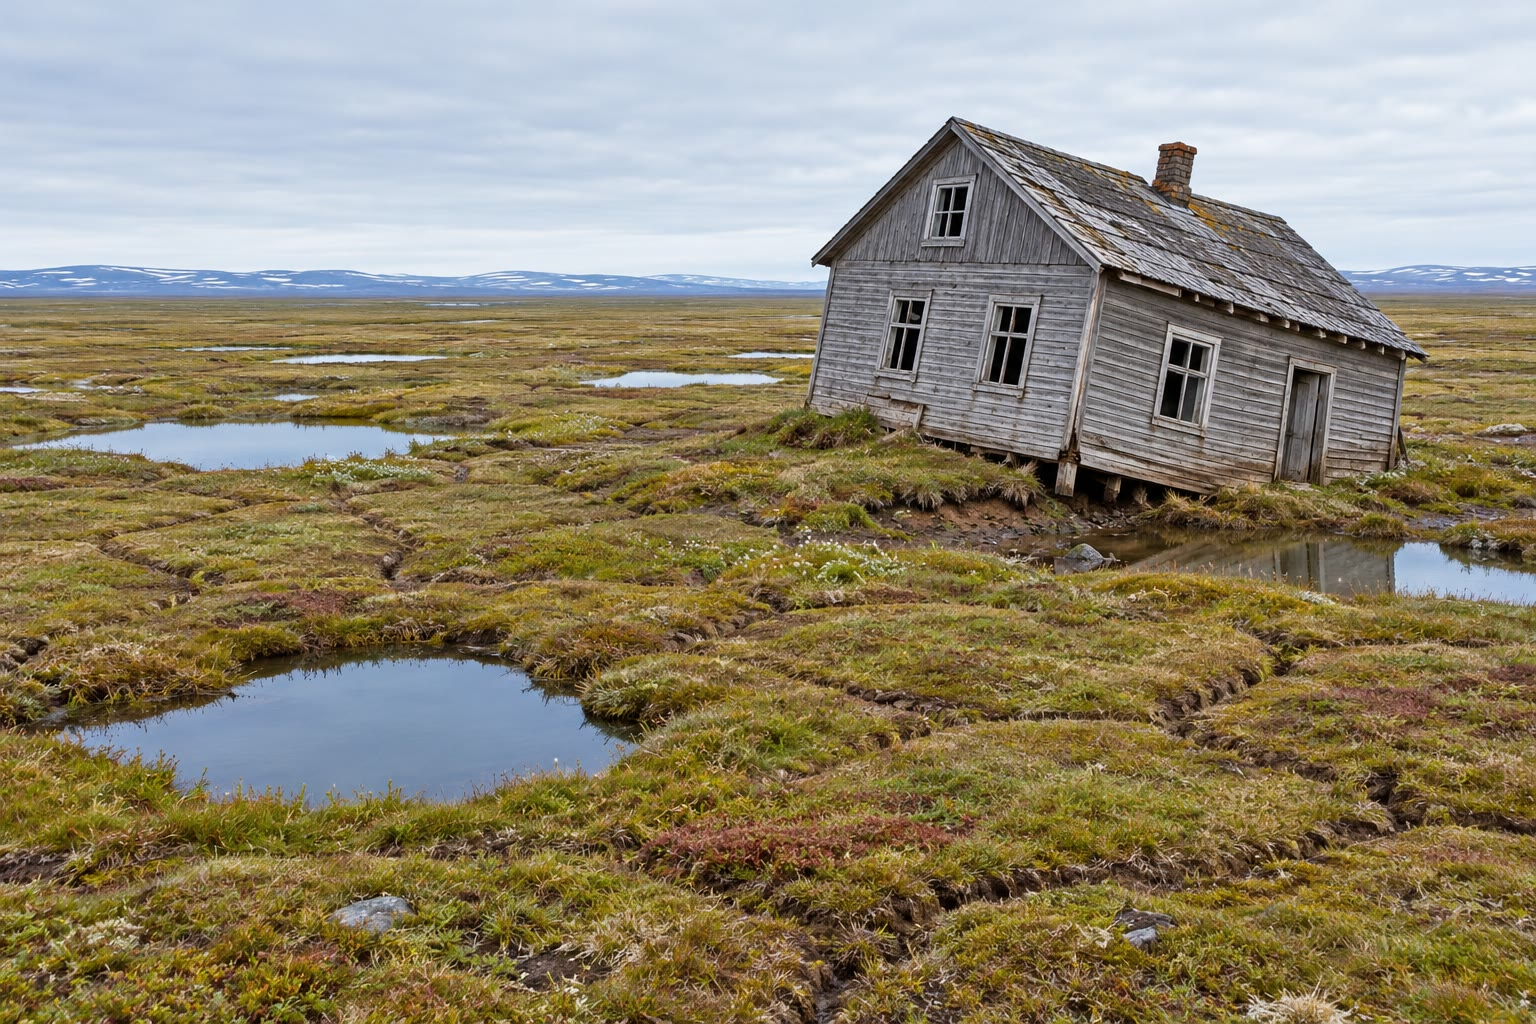
\includegraphics[width=\linewidth]{images/book1/ai/g8-permafrost-house.jpg}
\end{minipage}\hfill
\begin{minipage}[c]{0.46\linewidth}\centering
\begin{tikzpicture}[font=\footnotesize]
  \fill[omLithAlluv] (0,0) rectangle (3.2,-0.6);
  \fill[omIce!70!omLithShale] (0,-0.6) rectangle (3.2,-3.0);
  \foreach \x/\y in {0.4/-1.0, 1.5/-1.3, 2.6/-0.9, 0.9/-1.9, 2.1/-2.2, 0.5/-2.6, 2.8/-2.6}
    \fill[white] (\x,\y) ellipse (0.22 and 0.06);
  \fill[omLithShale!60] (0,-3.0) rectangle (3.2,-3.6);
  \draw[green!45!black, line width=1pt] (0,0) -- (3.2,0);
  \node[anchor=west, align=left] at (3.3,-0.3) {\textbf{الطبقة النشطة}\\ تذوب في\\ كل صيف};
  \node[anchor=west, align=left] at (3.3,-1.8) {\textbf{التربة الصقيعية}\\ متجمدة طوال السنة\\ وفيها عدسات جليد};
  \node[anchor=west, align=left] at (3.3,-3.3) {أرض غير\\ متجمدة};
\end{tikzpicture}
\end{minipage}

\smallskip
{\small يمينًا: بيت يميل فوق \omterm{def:g8:ice-on-earth:permafrost}{تربة صقيعية} تذوب في التندرا (رسم توضيحي
مولَّد بالذكاء الاصطناعي لمشهد عام). يسارًا: الأرض تحت التندرا (رسم
تخطيطي، ليس بمقياس رسم).}
\label{fig:g8:ice-on-earth:permafrost}
\end{omfigure}

\section{العصور الجليدية}

لم يغطِّ الجليد دائمًا الجزء نفسه من الأرض. فقبل نحو \num{20000} سنة، كانت
\omterm{def:g8:ice-on-earth:ice-sheet}{الأغطية الجليدية} تغطي جزءًا كبيرًا من أمريكا الشمالية وشمال أوروبا، بما فيه
إسكندينافيا. وكانت \omterm{def:g8:ice-on-earth:glacier}{الأنهار الجليدية} تغطي حينئذ نحو ربع اليابسة، مقابل نحو
عُشرها اليوم. وقد حُبس في هذا الجليد من الماء ما جعل \omterm{def:g2:water-on-earth:ocean}{البحر} أدنى من مستواه
اليوم بأكثر من \qty{120}{m}: فكانت أجزاء من الرفوف القارية الحالية أرضًا
يابسة. ومنذ نحو \num{15000} سنة أخذت \omterm{def:g8:ice-on-earth:ice-sheet}{الأغطية الجليدية} تذوب وتنحسر، وارتفع
\omterm{def:g2:water-on-earth:ocean}{البحر}؛ وبلغ مستواه الحالي تقريبًا قبل نحو \num{8000}
سنة.
% ledger: usgs:lgm, nsidc:ice-sheets, nsidc:ice-cover

\begin{definition}[العصر الجليدي]\label{def:g8:ice-on-earth:ice-age}
\emph{العصر الجليدي}\index{عصر جليدي} زمن بارد طويل في تاريخ الأرض تمتد فيه
\omterm{def:g8:ice-on-earth:ice-sheet}{الأغطية الجليدية} بعيدًا خارج المناطق القطبية وتغطي أجزاء كبيرة من \omterm{def:g3:continents-and-oceans:continent}{القارات}.
وقد بلغ آخر عصر جليدي أشد برودته قبل نحو \num{20000} سنة وانتهى قبل نحو
\num{12000} سنة.
\end{definition}
% ledger: usgs:lgm, nps:u-valley

دلائل آخر \omterm{def:g8:ice-on-earth:ice-age}{عصر جليدي} موجودة في كل مكان من الأراضي التي غطاها: \omterm{def:g1:landscapes-around-us:landform}{أودية} على شكل
حرف U بعيدة عن أي \omterm{def:g8:ice-on-earth:glacier}{نهر جليدي} اليوم، وركامات جليدية طرفية تعترض \omterm{def:g1:landscapes-around-us:landform}{السهول}، \omterm{def:g3:stones-pebbles-sand:rock}{وصخور}
ضالة قابعة في الحقول. ولم يكن العصر الوحيد. فعلى مدى بضع مئات الآلاف من السنين
الأخيرة، تعاقبت \omterm{def:g8:ice-on-earth:ice-age}{العصور الجليدية} والأزمنة الأدفأ التي بينها مرة بعد مرة؛ ونحن
نعيش في أحد الأزمنة الدافئة. ويروي \Cref{ch:g9:climate-past-and-present} كيف
يقرأ العلماء هذه القصة الطويلة في جليد القارة القطبية الجنوبية
نفسه.
% ledger: nps:u-valley, nps:moraines, usgs:erratic

\section{تمارين}

\begin{exercise}[$\star$]\label{exo:g8:ice-on-earth:1}
مستعينًا بالمقطع الطولي \omterm{def:g8:ice-on-earth:glacier}{للنهر الجليدي} في هذا الفصل، سمِّ: (أ) جزء \omterm{def:g8:ice-on-earth:glacier}{النهر
الجليدي} الذي يكسب فيه جليدًا؛ (ب) الجزء الذي يخسر فيه جليدًا؛ (ج) طرف \omterm{def:g8:ice-on-earth:glacier}{النهر
الجليدي} الأمامي؛ (د) الحاجز المرتفع من الحطام الصخري عند نهايته.
\end{exercise}

\begin{exercise}[$\star$]\label{exo:g8:ice-on-earth:2}
% ledger: nsidc:firn, nsidc:glacier-flow, nsidc:sea-ice-def
صواب أم خطأ؟ صحّح الجمل الخاطئة. (أ) يتكون \omterm{def:g8:ice-on-earth:glacier}{النهر الجليدي} من ماء \omterm{def:g2:water-on-earth:ocean}{بحر}
متجمد. (ب) يستغرق \omterm{def:g4:clouds-rain-snow:precipitation}{الثلج} نحو سنة ليصير ثلجًا حبيبيًا. (ج) حين يتراجع \omterm{def:g8:ice-on-earth:glacier}{النهر
الجليدي}، يجري جليده صعودًا. (د) يكون \omterm{def:g8:ice-on-earth:sea-ice}{الجليد البحري} في المنطقة القطبية الشمالية
في أصغر امتداد له في سبتمبر.
\end{exercise}

\begin{exercise}[$\star$]\label{exo:g8:ice-on-earth:3}
% ledger: usgs:erratic, nsidc:permafrost
أعطِ الكلمة المناسبة لكل وصف: (أ) \omterm{def:g1:landscapes-around-us:landform}{وادٍ} له قاع عريض وجوانب شديدة الانحدار،
نحته الجليد؛ (ب) جلمود حمله \omterm{def:g8:ice-on-earth:glacier}{نهر جليدي} بعيدًا عن موطنه؛ (ج) لوح من الجليد طافٍ
لا يزال متصلًا بالجليد على اليابسة؛ (د) أرض تبقى متجمدة مدة سنتين متتاليتين على
الأقل.
\end{exercise}

\begin{exercise}[$\star$]\label{exo:g8:ice-on-earth:4}
% ledger: nsidc:ice-sheets, nsidc:ice-cover
(أ) ما الأرضان اللتان تغطيهما اليوم \omterm{def:g8:ice-on-earth:ice-sheet}{أغطية جليدية}؟ (ب) أيهما ترفع \omterm{def:g2:water-on-earth:ocean}{البحر} أكثر لو
ذاب كل جليدها، وبكم؟ (ج) ما حصة اليابسة على الأرض التي يغطيها الجليد
اليوم؟
\end{exercise}

\begin{exercise}[$\star\star$]\label{exo:g8:ice-on-earth:5}
% ledger: data:b1-nsidc-sea-ice (figdata/grade-8/sea_ice.py)
استعمل مخطط \omterm{def:g8:ice-on-earth:sea-ice}{الجليد البحري} في المنطقة القطبية الشمالية في سبتمبر. (أ) اقرأ
الامتداد عام 1979 وعام 2012. (ب) بكم مليون~\babelsublr{km$^2$} تقلص بين هاتين
السنتين؟ (ج) ما الكسر الذي كان قد زال من امتداد عام 1979 بحلول عام 2012؟
قرّبه إلى كسر بسيط. (د) لماذا تكون مقارنة خط الاتجاه أوثق من مقارنة سنتين
منفردتين؟
\end{exercise}

\begin{exercise}[$\star\star$]\label{exo:g8:ice-on-earth:6}
% ledger: nsidc:muir, uw:pedersen
تراجعت مقدمة \omterm{def:g1:landscapes-around-us:water}{نهر} ميوير الجليدي \qty{12}{km} بين عامي 1941 و2004.
(أ) كم سنة هذه؟ (ب) ما متوسط تراجعه في السنة، بالأمتار؟ قرّب إلى أقرب عشرة
أمتار. (ج) تراجع \omterm{def:g1:landscapes-around-us:water}{نهر} بيدرسن الجليدي \qty{3.2}{km} بين عامي 1984 و2021. فما
متوسط تراجعه في السنة؟ (د) أي النهرين الجليديين تراجع
أسرع؟
\end{exercise}

\begin{exercise}[$\star\star$]\label{exo:g8:ice-on-earth:7}
اشرح، في بضع جمل وبالترتيب، كيف يصير \omterm{def:g4:clouds-rain-snow:precipitation}{الثلج} الساقط عاليًا على \omterm{def:g1:landscapes-around-us:landform}{جبل} جليدَ مقدمة
\omterm{def:g8:ice-on-earth:glacier}{نهر جليدي}، بعيدًا في أسفل \omterm{def:g1:landscapes-around-us:landform}{الوادي}. استعمل الكلمات \emph{\omterm{def:g4:clouds-rain-snow:precipitation}{الثلج} الحبيبي}،
و\emph{منطقة التراكم}، و\emph{يجري}، و\emph{منطقة
الذوبان}.
\end{exercise}

\begin{exercise}[$\star\star$]\label{exo:g8:ice-on-earth:8}
% ledger: nsidc:ice-shelves
تُملأ كأسان إلى المستوى نفسه. في الكأس A، تطفو مكعبات جليد على الماء؛ وفي
الكأس B، توضع مكعبات الجليد نفسها على حجر فوق الماء. (أ) بعد أن يذوب الجليد،
في أي الكأسين ارتفع المستوى؟ (ب) أي الكأسين نموذج \omterm{def:g8:ice-on-earth:ice-sheet}{لجبل جليدي} يذوب في \omterm{def:g2:water-on-earth:ocean}{البحر}؟
ولغطاء جليدي يذوب على اليابسة؟ (ج) لماذا يظل لتفكك \omterm{def:g8:ice-on-earth:ice-sheet}{الرف الجليدي} أثر في مستوى
\omterm{def:g2:water-on-earth:ocean}{البحر}؟
\end{exercise}

\begin{exercise}[$\star\star$]\label{exo:g8:ice-on-earth:9}
تعبر امرأة في نزهة سيرًا \omterm{def:g1:landscapes-around-us:landform}{واديًا} عريضًا قاعه مستوٍ وجوانبه شديدة الانحدار جدًا.
وفي وسط حقل تجد جلمودًا من الغرانيت بحجم سيارة؛ \omterm{def:g3:stones-pebbles-sand:rock}{وصخور} \omterm{def:g1:landscapes-around-us:landform}{الوادي} كلها من الحجر
الجيري. وفي موضع أعلى، يمتد حاجز طويل من الحجارة المختلطة على طول جانب \omterm{def:g1:landscapes-around-us:landform}{الوادي}.
(أ) ما شكل \omterm{def:g1:landscapes-around-us:landform}{الوادي}، وما الذي نحته؟ (ب) كيف وصل الجلمود إلى هناك؟ وما اسمه؟
(ج) ما هذا الحاجز، وماذا يخبرك ارتفاعه على جانب \omterm{def:g1:landscapes-around-us:landform}{الوادي}؟
\end{exercise}

\begin{exercise}[$\star\star$]\label{exo:g8:ice-on-earth:10}
% ledger: nsidc:ice-sheets
سيرفع \omterm{def:g8:ice-on-earth:ice-sheet}{الغطاء الجليدي} \omterm{def:g3:continents-and-oceans:continent}{للقارة} القطبية الجنوبية \omterm{def:g2:water-on-earth:ocean}{البحر} نحو \qty{58}{m} لو ذاب
كله، \omterm{def:g8:ice-on-earth:ice-sheet}{والغطاء الجليدي} لغرينلاند نحو \qty{7.4}{m}. (أ) كم يضيف عُشر جليد
غرينلاند؟ (ب) كم يضيف جزء من مئة من جليد القارة القطبية الجنوبية؟ (ج) كم مرة
يزيد ما تحتويه القارة القطبية الجنوبية على ما تحتويه غرينلاند؟ قرّب إلى أقرب
عدد صحيح.
\end{exercise}

\begin{exercise}[$\star\star\star$]\label{exo:g8:ice-on-earth:11}
% ledger: data:b1-nsidc-sea-ice (figdata/grade-8/sea_ice.py: mean_1980s, mean_2010s, trend)
كان متوسط امتداد \omterm{def:g8:ice-on-earth:sea-ice}{الجليد البحري} في المنطقة القطبية الشمالية في سبتمبر
\num{7.21}~مليون~\unit{km^2} على مدى السنوات 1980--1989
و\num{4.65}~مليون~\unit{km^2} على مدى السنوات 2010--2019. (أ) المليون يساوي
$10^6$. اكتب القيمتين بوحدة \babelsublr{km$^2$}، دون كلمة «مليون».
(ب) بكم انخفض متوسط الامتداد بين هذين العقدين؟
(ج) يفصل بين العقدين 30 سنة. فما الانخفاض في كل عقد؟
قارنه بانخفاض خط الاتجاه البالغ \num{0.76}~مليون~\unit{km^2} في كل عقد.
(د) لماذا لا يمكن مدّ خط اتجاه مستقيم إلى ما لا نهاية في
المستقبل؟
\end{exercise}

\begin{exercise}[$\star\star\star$]\label{exo:g8:ice-on-earth:12}
% ledger: usgs:lgm (the shelf slope is exercise data)
قبل نحو \num{20000} سنة كان \omterm{def:g2:water-on-earth:ocean}{البحر} أدنى من مستواه اليوم بنحو \qty{120}{m}.
وقبالة \omterm{def:g1:landscapes-around-us:water}{ساحل} ما، ينحدر \omterm{def:g8:the-oceans:seafloor}{الرف القاري} انحدارًا لطيفًا جدًا، بمقدار \qty{1}{m} لكل
\qty{1}{km} نحو عرض \omterm{def:g2:water-on-earth:ocean}{البحر} (بيانات التمرين). (أ) على أي بعد في عرض \omterm{def:g2:water-on-earth:ocean}{البحر} كان
\omterm{def:g1:landscapes-around-us:water}{الساحل} حينئذ؟ (ب) أين ذهب الماء الناقص، أي ما يعادل \qty{120}{m}؟ (ج) اشرح
لماذا يكون \omterm{def:g8:ice-on-earth:glacial-landforms}{الركام الجليدي} الطرفي الذي يوجد اليوم في \omterm{def:g1:landscapes-around-us:landform}{سهل}، بعيدًا عن أي \omterm{def:g1:landscapes-around-us:landform}{جبال}،
دليلًا على \omterm{def:g8:ice-on-earth:ice-age}{العصر الجليدي} نفسه.
\end{exercise}

\section{مسألة: تراجع طويل لنهر جليدي}

\begin{problem}[{مسألة نهاية الأسبوع --- قيست مقدمة نهر جليدي جبلي كل عشر
سنوات منذ 1960؛ تُحسب سرعة تراجعه، ويُقرأ الوادي الذي
يتركه}]
\label{pb:g8:ice-on-earth:1}
% ledger: nsidc:muir, uw:pedersen, nps:moraines (figdata/grade-8/glacier_retreat.py; Glacier G and its measurements are exercise data)
منذ 1960، يقيس فريق كل عشر سنوات موضع مقدمة \omterm{def:g8:ice-on-earth:glacier}{النهر الجليدي}~G، وهو \omterm{def:g8:ice-on-earth:glacier}{نهر جليدي}
في \omterm{def:g1:landscapes-around-us:landform}{وادٍ} بين \omterm{def:g1:landscapes-around-us:landform}{الجبال}. وتُقاس المسافة صعودًا في \omterm{def:g1:landscapes-around-us:landform}{الوادي} انطلاقًا من علامة
صخرية~R، طُليت على قاع \omterm{def:g1:landscapes-around-us:landform}{الوادي} عند المقدمة عام 1960. ويقوم كوخ~H بجانب قاع
\omterm{def:g1:landscapes-around-us:landform}{الوادي}، على بعد \qty{1980}{m} صعودًا في \omterm{def:g1:landscapes-around-us:landform}{الوادي} من~R. وتبين \omterm{def:g2:drawing-to-map:map}{الخريطة} المقدمة
عند كل قياس، والحاجز الواقع أسفل مقدمة عام 1960
مباشرة.

\begin{center}
\begin{tikzpicture}
\begin{axis}[axis equal image, width=12.5cm, xmin=-500, xmax=2600, ymin=-760, ymax=760,
  axis lines=none, clip=true]
  \fill[black!13] (axis cs:-500,-760) rectangle (axis cs:2600,760);
  \addplot[fill=white, draw=none] table[x=y, y=x] {figdata/out/grade-8-glacier_retreat-floor.dat} -- cycle;
  \addplot[fill=omIce, draw=none] table[x=y, y=x] {figdata/out/grade-8-glacier_retreat-ice.dat} -- cycle;
  \addplot[black!70, line width=0.8pt] table[x=y, y=x] {figdata/out/grade-8-glacier_retreat-walls.dat};
  \addplot[omCold, line width=0.9pt] table[x=y, y=x] {figdata/out/grade-8-glacier_retreat-fronts.dat};
  \addplot[omLithCongl!80!black, line width=3pt] table[x=y, y=x] {figdata/out/grade-8-glacier_retreat-moraine.dat};
  \addplot[only marks, mark=none, nodes near coords, point meta=explicit symbolic,
    every node near coord/.style={anchor=south, rotate=90, font=\scriptsize, inner sep=1pt}]
    table[x=y, y=x, meta=year] {figdata/out/grade-8-glacier_retreat-labels.dat};
  \addplot[only marks, mark=*, mark size=2pt] coordinates {(0,0)};
  \node[font=\footnotesize\bfseries, anchor=south east] at (axis cs:-10,10) {R};
  \addplot[only marks, mark=square*, mark size=2.6pt, omDef] coordinates {(1980,-560)};
  \node[font=\footnotesize\bfseries, anchor=north] at (axis cs:1980,-590) {H};
  \node[font=\scriptsize, anchor=west] at (axis cs:-480,-590) {\foreignlanguage{arabic}{$\longrightarrow$ نحو أعلى الوادي}};
  \node[font=\scriptsize] at (axis cs:2250,0) {\foreignlanguage{arabic}{الجليد في 2020}};
  \draw[black, line width=1.2pt] (axis cs:2000,640) -- (axis cs:2500,640)
    node[midway, below, font=\scriptsize] {\qty{500}{m}};
\end{axis}
\end{tikzpicture}

\smallskip
{\small
\begin{tabular}{|l|c|c|c|c|c|c|c|}
\hline
السنة & 1960 & 1970 & 1980 & 1990 & 2000 & 2010 & 2020 \\
\hline
بعد المقدمة عن R \babelsublr{(m)} & 0 & 180 & 330 & 520 & 700 & 880 & 1080 \\
\hline
\end{tabular}}
\end{center}

\noindent\textbf{الجزء الأول --- مواضع المقدمة.}\par\nopagebreak
\begin{enumerate}[beginpenalty=10000]
  \item كم تراجعت المقدمة بين 1960 و2020؟
  \item احسب مقدار تراجعها في كل عقد. في أي عقد كان تراجعها أقل ما
        يكون؟ وأكبر ما يكون؟
  \item هل توقف \omterm{def:g8:ice-on-earth:glacier}{النهر الجليدي} عن الجريان نحو الأسفل؟ علّل.
  \item الحاجز الداكن الواقع أسفل مقدمة عام 1960 مباشرة مكوَّن من حطام
        صخري مختلط. ما اسمه، وكيف تكوّن؟
\end{enumerate}

\noindent\textbf{الجزء الثاني --- سرعة التراجع.}\par\nopagebreak
\begin{enumerate}[resume, beginpenalty=10000]
  \item ما متوسط التراجع في كل عقد بين 1960 و2020؟
  \item وفي كل سنة؟
  \item تراجع \omterm{def:g1:landscapes-around-us:water}{نهر} ميوير الجليدي \qty{12}{km} في 63 سنة، أي نحو
        \qty{190}{m} في السنة. فكم مرة كان ذلك أسرع من \omterm{def:g8:ice-on-earth:glacier}{النهر
        الجليدي}~G؟
  \item هل كسب \omterm{def:g8:ice-on-earth:glacier}{النهر الجليدي}~G في منطقة تراكمه من الجليد أكثر مما خسر
        في منطقة ذوبانه، أم أقل؟ علّل.
\end{enumerate}

\noindent\textbf{الجزء الثالث --- الوادي الذي يتركه.}\par\nopagebreak
\begin{enumerate}[resume, beginpenalty=10000]
  \item أي شكل تتوقع أن يكون لقاع \omterm{def:g1:landscapes-around-us:landform}{الوادي} بين R ومقدمة عام 2020 في
        مقطع عرضي؟ لماذا؟
  \item في عام 2020، كم كانت المقدمة تبعد عن مستوى الكوخ؟
  \item بالسرعة المتوسطة التي في الجزء~الثاني، كم سنة تحتاج المقدمة
        لتبلغ مستوى الكوخ؟ وفي أي سنة يكون ذلك؟
  \item اذكر سببًا واحدًا يجعل هذه السنة ليست تنبؤًا.
\end{enumerate}
\end{problem}
